% Number 340
% CAPMG Units
% Graph conversion a->v->x
% JG

% Watermark
\AddToShipoutPicture*{\BackgroundPic}

\addtocounter {ProbNum} {1}

%\begin{floatingfigure}[r]{.3\textwidth}
%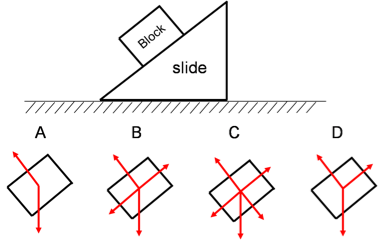
\includegraphics[scale=.4]{/Users/jgates/desktop/latex/pics/incline3.png}
%\end{floatingfigure}
 
{\bf \Large{\arabic{ProbNum}}} Draw the position and velocity graphs that correspond to the given acceleration graph, initial position of -3 meters, and initial velocity of ${2~\tfrac{m}{s}}$.

\begin{center}
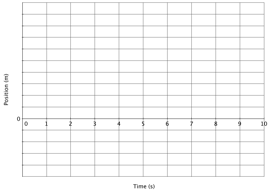
\includegraphics[scale=1]{/Users/jgates/desktop/latex/pics/blankxgraph2.png}
\end{center}

\begin{center}
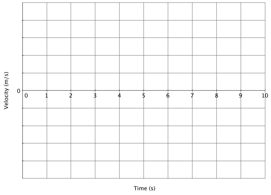
\includegraphics[scale=1]{/Users/jgates/desktop/latex/pics/blankvgraph2.png}
\end{center}

\begin{center}
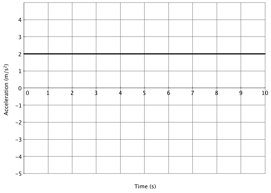
\includegraphics[scale=1]{/Users/jgates/desktop/latex/pics/givenagraph2.png}
\end{center}


\vfill
\newpage
